\documentclass{vc}

% タイトルの定義(最初のページの上部に出力されるほか、PDFのメタデータとしても利用される)
\title{Visual Computing論文テンプレート}

% 著者の定義(PDFのメタデータとして利用される)
\plainauthors{画像 花子, 電子 太郎, 学会 三郎}

% 著者の定義(最初のページの上部に出力される)
\begin{authors}
  % 固定幅かつセンタリングのカラム "C" の定義(幅は著者数や文字数に応じて各自調整する)
  % Reference: https://en.wikibooks.org/wiki/LaTeX/Tables
  \newcolumntype{C}{>{\centering}p{0.20\textwidth}}

  % 上記のカラム定義 "C" を用いた表の定義(二行以上必要な場合等のレイアウトは各自調整する)
  \begin{tabular}{CCC}
    画像 花子$^\dagger$ & 電子 太郎$^\ddagger$ & 学会 三郎$^\ddagger$
  \end{tabular}
\end{authors}

% 著者所属の定義(最初のページの上部に出力される)
\begin{affiliations}
  \begin{tabular}{cc}
    $\dagger$画像大学工学部 & $\ddagger$画像株式会社開発部
  \end{tabular}
\end{affiliations}

% 著者メールアドレスの定義(最初のページの上部に出力される)
\begin{emails}
  \begin{tabular}{c}
    E-mail: $\dagger${}hanako@gazo.ac.jp, $\ddagger${}\{taro, saburo\}@denshi.co.jp
  \end{tabular}
\end{emails}

% 概要の定義(最初のページのタイトルの直後に出力される)
\begin{abstract}
  本テンプレートは, コンピュータグラフィクス及びその周辺分野における技術に関する学術シンポジウムVisual Computingへの投稿原稿を執筆するために作成されたものである.
\end{abstract}

% ティザー画像の定義(最初のページの上部に出力される)
% Note: 不要な場合はteaserfigure環境ごと削除する
\begin{teaserfigure}
  \centering
  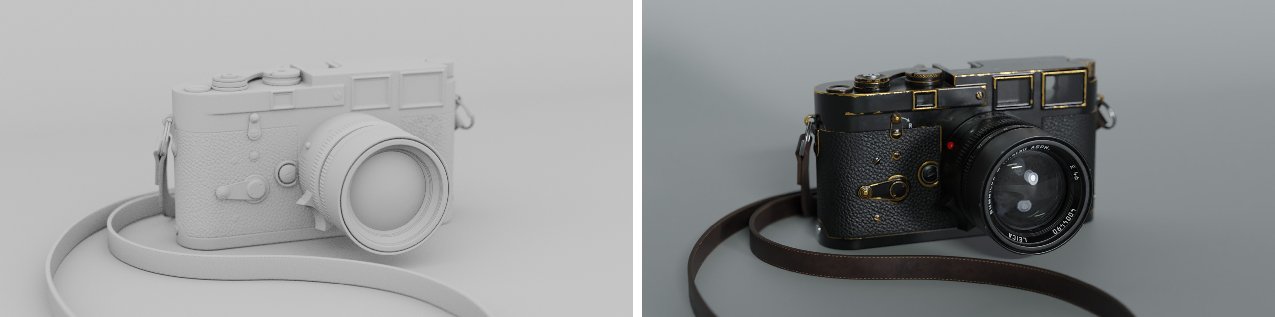
\includegraphics[width=\textwidth]{./figures/leica.pdf}
  \caption{ティザー画像のキャプションをここに記述する.}
  \label{fig:teaser}
\end{teaserfigure}

\begin{document}

\maketitle

% ------------------------------------------------------------------------------
% 以下に論文本文を記述する
% ------------------------------------------------------------------------------

\section{原稿作成における注意事項}

投稿時の原稿には著者名, 所属, 謝辞などは一切記入しないでください.
WordからPDFを作成した場合, 文書のプロパティに著者を特定できる情報が入ることがありますが, そのような情報は削除してください.

\section{テンプレートの使用例}
\label{sec:template}

本テンプレートを用いて原稿の本文を記述する際の例を下記に示す.
なお表の詳細なフォーマットや参照に用いるコマンド\footnote{ここでは\textsf{cleveref}パッケージが提供する\textsf{cref}コマンド\cite{Wikibooks:LaTeX:Ref}を利用している.}などは厳密に従う必要はない.

インライン数式は$\mathbf{x} \in \mathbb{R}^{n}$のように記述する.
ディスプレイ数式は
\begin{align}
  \mathbf{x}^{*} = \mathop{\text{arg max}}_{\mathbf{x} \in \mathcal{X}} f(\mathbf{x})
  \label{eq:optimization}
\end{align}
などのように記述する.
数式は\cref{eq:optimization}などのように参照する.
図は\cref{fig:teaser}や\cref{fig:leica}などのように参照する.
表は\cref{tab:accuracy}などのように参照する.
セクションは\cref{sec:template}などのように参照する.
参考文献は\cite{GSC12,WL00}などのように参照する.
URLは\url{https://www.siggraph.org/}のように記載する.

\begin{figure}
  \centering
  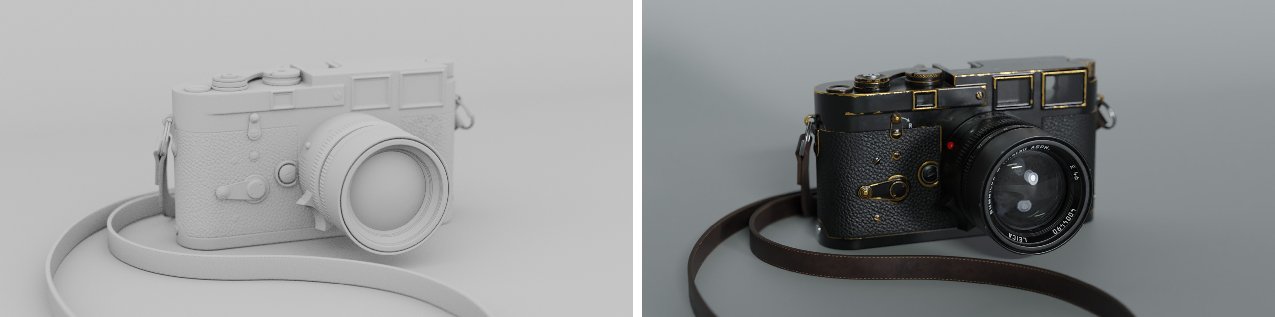
\includegraphics[width=\columnwidth]{./figures/leica.pdf}
  \caption{図のキャプションをここに記述する.}
  \label{fig:leica}
\end{figure}

\begin{table}
  \centering
  \caption{表のキャプションをここに記述する.}
  \label{tab:accuracy}
  \begin{tabular}{@{}rrrr@{}}
    \toprule
    & Our method & XXX et al. & YYY et al. \\
    \midrule
    Case 1 & \textbf{95.4\%} &         91.2\%  & 92.4\% \\
    Case 2 & \textbf{97.5\%} &         92.1\%  & 91.2\% \\
    Case 3 &         90.3\%  & \textbf{90.9\%} & 82.5\% \\
    \midrule
    Mean   & \textbf{94.4\%} &         91.4\%  & 88.7\% \\
    \bottomrule
  \end{tabular}
\end{table}

\section{テンプレートの詳細}

\subsection{テンプレートの実装}

\textsf{vc}クラスファイルは\textsf{bxjsarticle}クラスファイルを基礎としており, pLaTeX, upLaTeX, LuaLaTeXでの利用をサポートしている.
このクラスファイルでは次のパッケージをロードしている:
\textsf{url},
\textsf{hyperref},
\textsf{hypcap},
\textsf{booktabs},
\textsf{graphicx},
\textsf{xcolor},
\textsf{amsmath},
\textsf{amssymb},
\textsf{array},
\textsf{natbib},
\textsf{bxpapersize},
\textsf{environ}.

\subsection{Overleaf環境での使用}

本テンプレートはローカル環境での使用に加えてオンライン環境の一つであるOverleaf\footnote{\url{https://www.overleaf.com/}}での使用もサポートしている.
Overleafで使用する場合, \cref{fig:overleaf}のように``New Project''メニュー下にある``Upload Project''項目を選択\footnote{ここでは2021年3月時点でのユーザインタフェースに基づき説明している.}し, 予めダウンロードしておいた本テンプレートのZIPファイルをアップロードする.

\begin{figure}
  \centering
  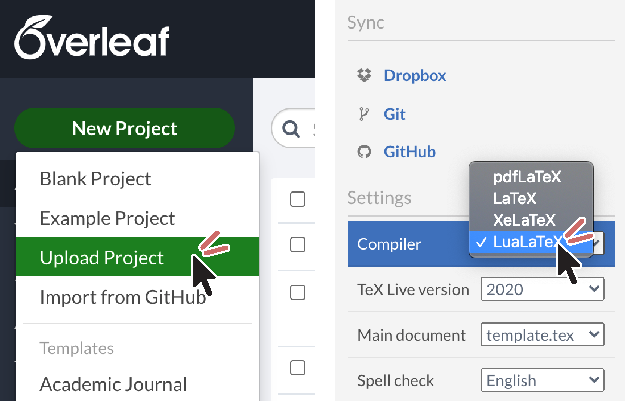
\includegraphics[width=.5\columnwidth]{./figures/overleaf.pdf}
  \caption{Overleafで本テンプレートを使用する際の手続き.}
  \label{fig:overleaf}
\end{figure}

\subsection{バグ報告・改善提案}

本テンプレートはGitHub\footnote{\url{https://github.com/visual-computing-symposium/paper-template}}上で管理されている.
バグ報告や改善提案などはGitHubを通して誰でも行うことができる.

\bibliographystyle{IEEEtran}
\bibliography{template.bib}

\end{document}
